\documentclass{article}
\title{CS 551 Project 1 Report}
\author{Group 20 \\\\ Ryan Attard, Sean Wallace,Velin Sedlarski,Adrian Birylo\\\\}
\date{October 25, 2013}

\usepackage{fullpage}
\usepackage{enumerate}

\usepackage{graphicx}

\usepackage{fancyvrb}
\DefineVerbatimEnvironment{code}{Verbatim}{fontsize=\small}
\DefineVerbatimEnvironment{example}{Verbatim}{fontsize=\small}
\newcommand{\ignore}[1]{}

\usepackage[usenames]{color}
\usepackage{listings}
\lstset{ %
	language=bash,                			% choose the language of the code
	basicstyle=\footnotesize,       			% the size of the fonts that are used for the code
	numbers=left,                   			% where to put the line-numbers
	numberstyle=\footnotesize,				% the size of the fonts that are used for the line-numbers
	stepnumber=1,                   			% the step between two line-numbers. If it is 1 each line will be numbered
	numbersep=5pt,                  			% how far the line-numbers are from the code
	backgroundcolor=\color{white},			% choose the background color. You must add \usepackage{color}
	showspaces=false,               			% show spaces adding particular underscores
	showstringspaces=false,         			% underline spaces within strings
	showtabs=false,                 			% show tabs within strings adding particular underscores
	frame=single,                   			% adds a frame around the code
	tabsize=2,              					% sets default tabsize to 2 spaces
	captionpos=t,	                   		% sets the caption-position to bottom
	breaklines=true,        					% sets automatic line breaking
	breakatwhitespace=false,    				% sets if automatic breaks should only happen at whitespace
	escapeinside={\%}{)}          			% if you want to add a comment within your code
}

\begin{document}
\maketitle
\pagebreak 
\section{API}

\subsection{int IGInit()}
This function initializes the framework by resetting all variables to that of their default values (namely 0).  The information is stored in static global variables, so any process which calls this will reset all of the data for each process.  In general, this function need not be called as the default values will be fine for the entirety of execution.  This function always returns 0.

\subsection{int IGLookup()}
This function copies the global storage array for all interest groups back to the calling process.  This is done using the \verb+sys_datacopy+ system call.  This function always returns 0.

\subsection{int IGCreate()}
This function creates a new interest group.  The identifier of the group is calculated using an auto incremented value.  The name of the group (string) is passed in through the \verb+sys_datacopy+ system call.  There is an upper limit to the number of interest groups we allow, so this function will return -1 if that limit has been reached and an interest group cannot be added, 0 otherwise.

\subsection{int IGPublisher()}
This function registers a process as a publisher within a given interest group.  It takes as argument the process ID of the requesting process and the ID of the interest group it wishes to join.  In the event it specifies an invalid interest group, the function returns -1.  If the process is already a publisher, then it returns -2.  Otherwise, it returns 0 and registers the process as a publisher.

\subsection{int IGSubscriber()}
This function registers a process as a subscriber within a given interest group.  It takes as argument the process ID of the requesting process and the ID of the interest group it wishes to join.  In the event it specifies an invalid interest group, the function returns -1.  If the process is already a subscriber, then it returns -2.  Otherwise, it returns 0 and registers the process as a publisher.

\subsection{int IGPublish()}
This function publishes a message to a specified interest group.  It takes as argument the sending PID, the destination process id, and a message represented as a character array.  As always, this information is taken from the message passed in from the system call.  If the specified interest group is nonexistent, it returns -1.  If there are already too many messages waiting, it returns -2.  If the requesting process is not a publisher, it returns -3.  Otherwise, the message is published to the interest group and returns 0.

\subsection{int IGRetrieve()}
This is the most complicated function of the group.  It takes as argument the requesting PID, the interest group of choice, and a message buffer to be populated by the function.  If the specified interest group is invalid, the function return -1.  If the requesting PID is not a subscriber, it returns -4.  If there are no messages to be retrieved, it returns -3.  If all of the messages for the given interest group have already been read by the given process, it returns -2.

If none of these are the case, then the function first checks to see which message to return to the client.  It does this by starting in the first index of the messages array present in the interest group structure.  Checking one by one, it continues until it either finds a message that has not yet been picked up by this process or until it has exhausted all options.

In the event it finds a message, this message is marked as read by this process and then the function checks to see if all other processes which are marked as subscribers for this interest group have picked up this message.  If they have not, the message is simply returned to the client.  If they have, the message is removed from the interest group entirely.


\section{Design}
The design of the IPC system call is such that it was added to the Process Management (PM) service. Below is a block diagram of how the IPC is implemented and what is in the user space and what is a service and in the kernel space. 

\begin{figure}[!h]
\center{
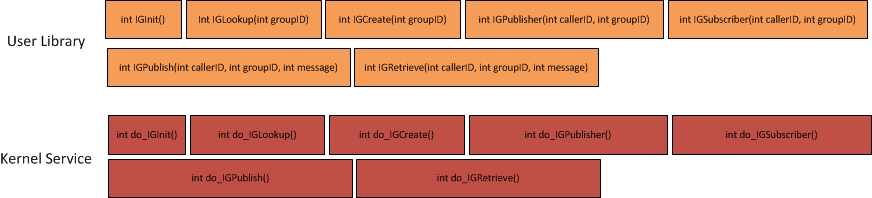
\includegraphics[width=\textwidth]{FlowChart.png}
\caption{Flow Chart}
}
\end{figure}

\section{Discussion}
In general deadlock can not occur since there are no blocking calls but a poorly written program can go into deadlock. Since there is no blocking calls a process is never waiting to get or put data in the IPC. Since the calls are not blocking they can fail and it is the responsibility of the programmer to make sure to recover from a failure gracefully and retry. 

\section{Test Cases}

There are a number of test cases which test all aspects of the system:

\begin{enumerate}
	\item testOverfillIG - Generates $ n $ interest groups where $ n $ is equal to the max supported.  It then tries to generate one more.  This should of course fail.  If it does, the function returns success.  If it fails at any point along the way, a failure notice is generated.
	\item testAlreadyPublisher - Creates an interest group, adds a publisher, then tries to add the same publisher once again.  If it does not, the function returns success.  If it fails at any point along the way, a failure notice is generated.
	\item testNotPublisher - Creates an interest group and tries to publish a message without having registered as a publisher first.  If the message does not post then it returns success. If it fails at any point along the way, a failure notice is generated.
	\item testPublisherInvalidInterestGroup - Creates a publisher and tries to publish to an invalid group.  If it does not, the function returns success.  If it fails at any point along the way, a failure notice is generated.
	\item testAlreadySubscriber - Identical to testAlreadyPublisher except for a subscriber.
	\item testNotSubscriber - Identical to testNotPublisher except for a subscriber.
	\item testSubscribeInvalidInterestGroup - Identical to testPublisherInvalidInterestGroup except for a subscriber.
	\item testRetriveNoMessages - Creates an interest group and a registers a subscriber.  It then tries to retrieve when there are no messages that have been posted.  If no messages are returned, the function returns success.  False otherwise.
	\item testAlreadyRetrivedAllMessages - Creates an interest group and registers a subscriber and a publisher and publishes a message.  This message is subsequently read by the subscriber a first time then tries to read it a second time.  Because there is only one message, no message should be returned on the second attempt.  If none is, it returns success, false otherwise.
	\item testOverfillMessages - Creates an interest group and a publisher.  The publisher then proceeds to publish 5 messages and then tries to publish one more.  Since the maximum is 5, the first 5 should succeed and the last should fail.  If this is the case, it returns success, false otherwise.
	\item testMessageDelete - Creates an interest group, a publisher, and two subscribers.  The publisher pushes two messages to the interest group and the subscribers then read these messages.  After the messages are read, they are checked to be deleted from the interest group.  If so, the function returns success, false otherwise.
	\item testMessageOrder - Creates an interest group, a publisher, and two subscribers.  The publisher pushes three messages to the interest group and the first subscriber checks all three.  The tests checks to make sure the messages received were in order and were not removed (as there is still another subscriber that has not checked these messages yet).  The second subscriber then checks all three messages and then the test function checks to make sure that all the messages were removed from the interest group.
\end{enumerate}

\section{Running the Code}

This is made very easy by a Makefile.  The image contains everything that is necessary to run the project.  Simply change directories into the ``Project2" directory, make, reboot, and then run \verb+./test+ inside the Project2 folder.

\end{document}
